\appendix
\renewcommand{\thetable}{IS\arabic{table}}%

\chapter{On the strength of hydrogen bonding within water clusters on the coordination limit}\label{paper2020}

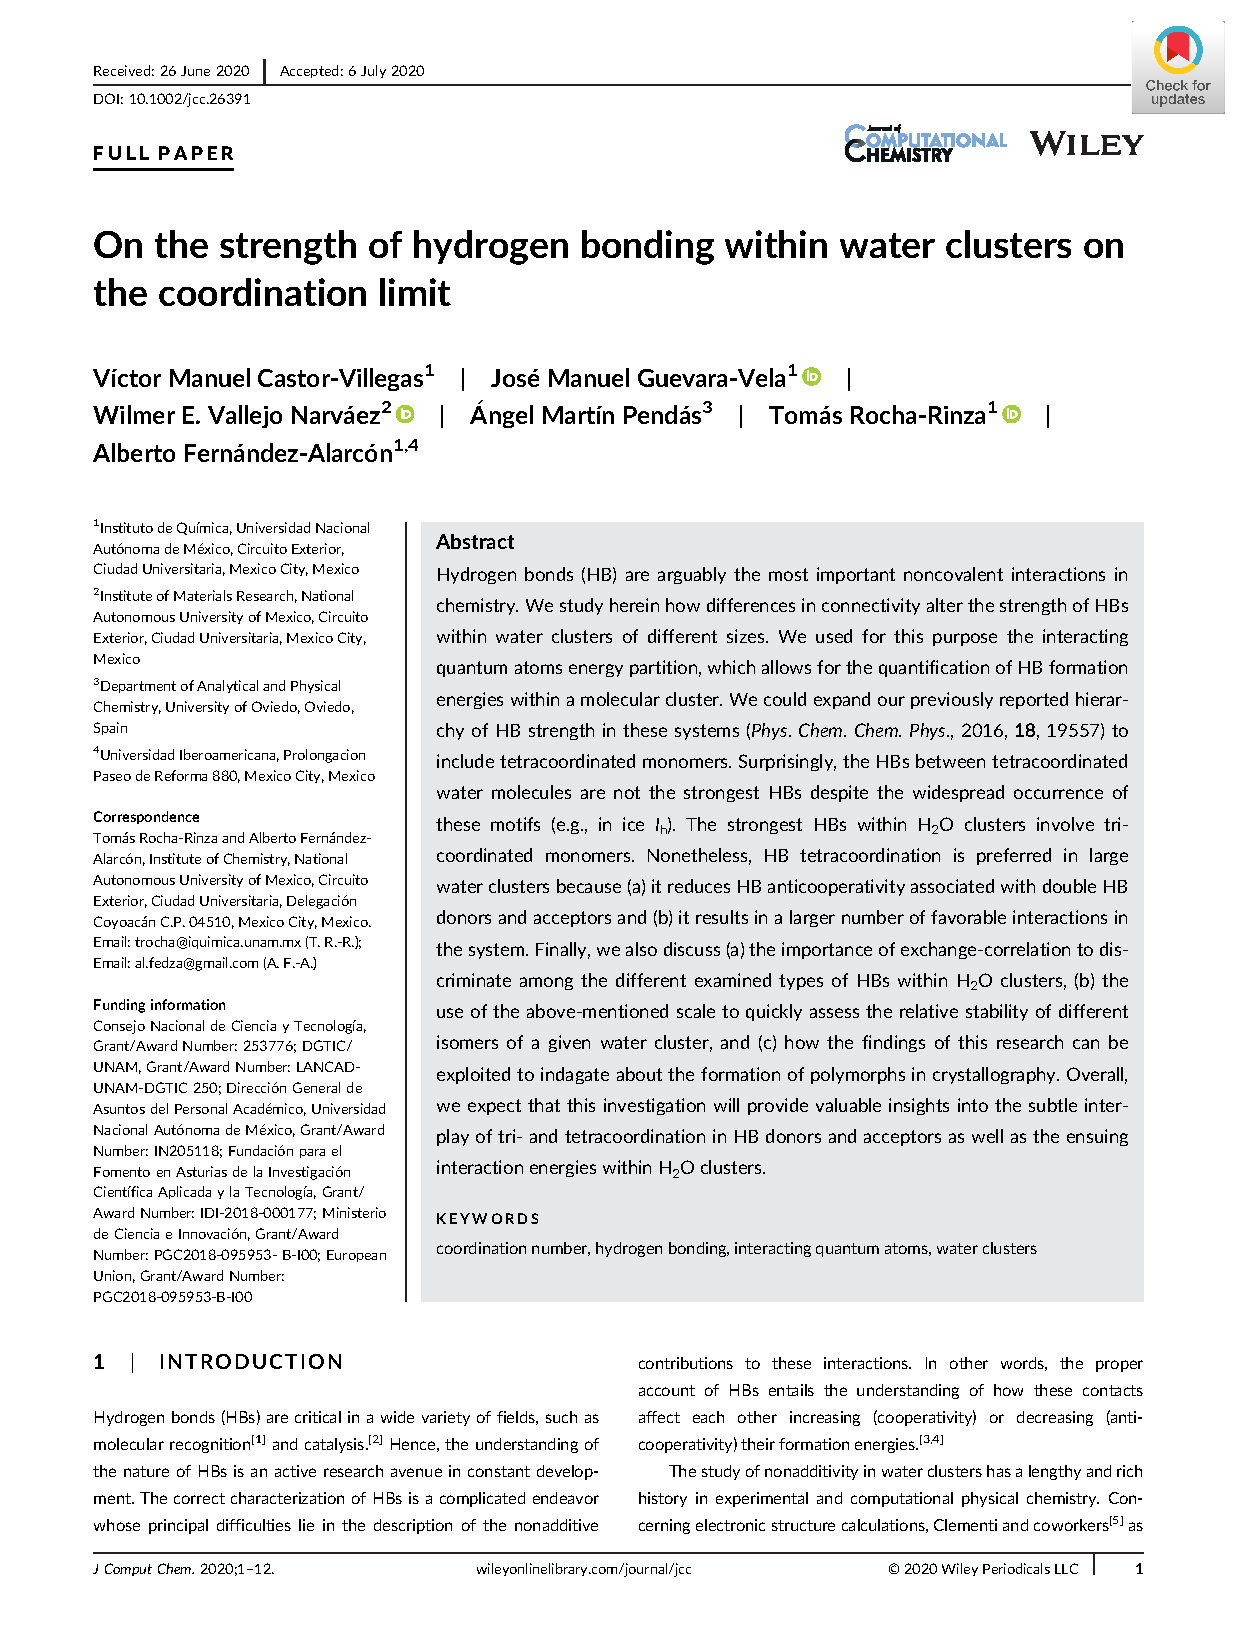
\includepdf[pages=-]{jcc26391}

\chapter{Información suplementaria}

\section{Geometrías al equilibrio para cúmulos de agua}

Coordenadas en \SI{}{\angstrom} de los cúmulos optimizados, formato xyz:

{\renewcommand{\baselinestretch}{.5}
\scriptsize{
\noindent \ce{(H_2O)_6} isómero bolsa
\VerbatimInput{./data_paper/6_bag.xyz}
\noindent  \ce{(H_2O)_6} isómero libro
\VerbatimInput{./data_paper/6_book.xyz}
\newpage
\noindent \ce{(H_2O)_6} isómero jaula
\VerbatimInput{./data_paper/6_cage.xyz}
\ce{(H_2O)_6} isómero prisma
\VerbatimInput{./data_paper/6_prism.xyz}
\ce{(H_2O)_6} isómero anillo
\VerbatimInput{./data_paper/6_ring.xyz}
\ce{(H_2O)_{10}} isómero 1
\VerbatimInput{./data_paper/10_H2O_1.xyz}
\ce{(H_2O)_{10}} isómero 2
\VerbatimInput{./data_paper/10_H2O_2.xyz}
\ce{(H_2O)_{10}} isómero 3
\VerbatimInput{./data_paper/10_H2O_3.xyz}
\ce{(H_2O)_{11}} isómero 1
\VerbatimInput{./data_paper/11_H2O_1.xyz}
\ce{(H_2O)_{11}} isómero 2
\VerbatimInput{./data_paper/11_H2O_2.xyz}
\ce{(H_2O)_{12}}
\VerbatimInput{./data_paper/12_H2O.xyz}
\newpage
\noindent \ce{(H_2O)_{13}}
\VerbatimInput{./data_paper/13_H2O.xyz}
\noindent \ce{(H_2O)_{14}}
\VerbatimInput{./data_paper/14_H2O.xyz}
\newpage
\noindent \ce{(H_2O)_{15}}
\VerbatimInput{./data_paper/15_H2O.xyz}
\ce{(H_2O)_{16}}
\VerbatimInput{./data_paper/16_H2O.xyz}
\ce{(H_2O)_{17}}
\VerbatimInput{./data_paper/17_H2O.xyz}}
}
\normalsize
\newpage

\section{$E_{\mathrm{int}}^{\mathscr{GH}\, \prime}$, distancias oxígeno-oxígeno
e índices de deslocalización para los distintos tipos de Enlace de Hidrógeno}

\begin{table}[h]
  \centering
    \caption{Promedio de valores para la energía de interacción
    $E_{\mathrm{int}}^{\mathscr{GH}\, \prime}$ (Ecuación \ref{eintprima}), sus
    contribuciones clásicas y de intercambio-correlación (Ecuación
    \ref{eint_cl_xc_prima}), la energía estimada $E_{\mathrm{HB}}$ (Ecuación
    \ref{estimada_eq}). También se reportan las distancias oxígeno-oxígeno (de las
    moléculas que interactúan mediante un EH), el índice de deslocalización y las
    desviaciones estándar de cada una de las cantidades presentadas en la tabla.
    Todas las energías reportadas están en \SI{}{\kilo\calorie\per\mole}, las
    distancias en \SI{}{\angstrom} y los índices de deslocalización en unidades
    atómicas.}
  \begin{adjustbox}{max width=1.1\textwidth,center}
  \scriptsize
    \begin{tabular}{c|cc|cc|cc|cc|cc|cc}
    \hline
    Tipo de EH & $E_{\mathrm{int}}^{\mathscr{GH'}}$ & $\sigma$ 
    & $E_{\mathrm{xc}}^{\mathscr{GH'}}$ & $\sigma$ & $E_{\mathrm{cl}}^{\mathscr{GH}'}$ &
    $\sigma$ & DI    & $\sigma$ & $E_\mathrm{HB}$ & $\sigma$ & O $\cdots$ O & $\sigma$ \\
    \hline
    10         & $-$9.551 & 0.551 & $-$6.831 & 0.436    & $-$2.720  & 0.126    & 0.234 & 0.019    & $-$15.077 & 2.255	& 2.646	& 0.032 \\
    9          & $-$8.692 & 0.660 & $-$6.122 & 0.486    & $-$2.569  & 0.179    & 0.203 & 0.017    & $-$11.716 & 1.905	& 2.699 & 0.034 \\
    8          & $-$8.570 & 0.329 & $-$5.930 & 0.225    & $-$2.641  & 0.107    & 0.196 & 0.010    & $-$11.327 & 0.953	& 2.715 & 0.020 \\
    7          & $-$7.829 & 0.035 & $-$5.546 & 0.234    & $-$2.282  & 0.226    & 0.190 & 0.006    & $-$10.440 & 0.299	& 2.723 & 0.013 \\
    6          & $-$7.340 & 0.633 & $-$5.036 & 0.487    & $-$2.305  & 0.196    & 0.182 & 0.016    & $-$9.610  & 1.349	& 2.757 & 0.025 \\
    5          & $-$6.927 & 0.575 & $-$4.930 & 0.424    & $-$1.997  & 0.317    & 0.175 & 0.013    & $-$9.091  & 1.217	& 2.745 & 0.030 \\
    4          & $-$6.947 & 0.524 & $-$4.852 & 0.483    & $-$2.095  & 0.175    & 0.166 & 0.019    & $-$8.605  & 1.727	& 2.776 & 0.050 \\
    3          & $-$6.410 & 1.088 & $-$4.628 & 0.517    & $-$1.782  & 0.612    & 0.161 & 0.016    & $-$7.875  & 2.169	& 2.760 & 0.040 \\
    2          & $-$6.165 & 0.458 & $-$4.121 & 0.293    & $-$2.043  & 0.243    & 0.151 & 0.010    & $-$7.147  & 0.833	& 2.799 & 0.034 \\
    1          & $-$5.804 & 0.912 & $-$3.905 & 0.510    & $-$1.899  & 0.470    & 0.141 & 0.017    & $-$6.466  & 1.235	& 2.849 & 0.046 \\
    \hline
    \end{tabular}
  \end{adjustbox}
\end{table}

\newpage
\thispagestyle{empty}
